\documentclass{beamer}
\usepackage[T1]{fontenc}
\usepackage[utf8]{inputenc}
\usepackage{lmodern}
\usepackage[ngerman]{babel}

\usepackage{graphics}

\usepackage{amsmath}
\usepackage{booktabs}
\usepackage{listings}

\usepackage{dot2texi}
\usepackage{tikz}
\usetikzlibrary{arrows,shapes}
 \usetikzlibrary{matrix}
\usetikzlibrary{automata}

\usepackage{wrapfig}

\usetheme{Singapore}
\usecolortheme{dove}
\graphicspath{{images/}{../comics/}}

\newcommand{\xn}{\visible<2->{$\times$}}
\newcommand{\xj}{\visible<2->{$\checkmark$}}
\newcommand{\rd}[1]{\textcolor{red}{#1}}
\newcommand{\gn}[1]{\textcolor{green}{#1}}
\newcommand{\bl}[1]{\textcolor{blue}{#1}}

\newcommand{\hiddencell}[2]{\action<#1->{#2}}

\newcommand{\link}[2][blue]{\underline{\textcolor{#1}{#2}}}
\renewcommand{\emph}[1]{\textit{\textcolor{gray}{#1}}}
\newcommand{\warn}[1]{\textcolor{red}{#1}}
\newcommand{\ans}[2]{\visible<#1->{\textcolor{green!70!black}{#2}}}
\newcommand{\wrong}[2]{\visible<#1->{\textcolor{red!70!black}{#2}}}
\newcommand{\xb}[1]{{\bf #1}}   % \xb {fett}
\newcommand{\xu}{\underline}    % \xu {unterstrichen}
\newcommand{\hide}{\onslide+<+(1)->}

\AtBeginSection[]
{
  \begin{frame}[plain]
    \frametitle{}
    {\footnotesize
      \tableofcontents[currentsection]
    }
  \end{frame}
}

\title{Grundbegriffe der Informatik}
\author{Patrick Niklaus}

\begin{document}
\begin{frame}
  \frametitle{Grundbegriffe der Informatik}
  \framesubtitle{13. Tutorium (letztes!)}
  \begin{description}
    \item \textbf{Name:} Patrick Niklaus
    \item \textbf{E-Mail:} patrick.niklaus@student.kit.edu
    \item \textbf{Nr:} 43
  \end{description}
\end{frame}

\section{Übungsblatt}
\begin{frame}
  \frametitle{Anmerkungen zum letzten Übungsblatt}
  \begin{enumerate}
    \item Eine Turingmachinen Konfiguration beinhaltet immer: Band, Zustand, Kopfposition
    \item Bei Akzeptoren: Jail/Müllzustand in der Klausur dazu malen.
  \end{enumerate}
\end{frame}

\section{Klausuren}
\begin{frame}
  \frametitle{Alte Klausuren für (fast) alle!}
\end{frame}

\section{Abschluss}
\subsection{xkcd}
\begin{frame}[plain]
  \begin{figure}
    \begin{center}
      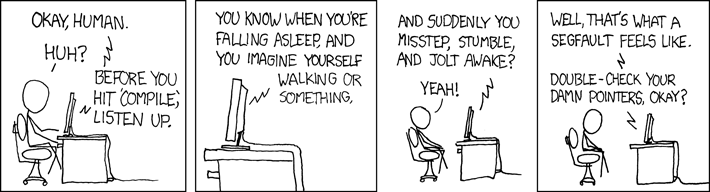
\includegraphics[width=300pt]{compiler_complaint}
    \end{center}
  \end{figure}
\end{frame}

\end{document}
